\documentclass[11pt]{article}
\usepackage[margin=1in]{geometry}
\usepackage[T1]{fontenc}
\usepackage[utf8]{inputenc}
\usepackage{lmodern,microtype}
\usepackage{amsmath,amssymb,amsthm,mathtools}
\usepackage{graphicx,booktabs,array,enumitem,setspace,placeins}
\usepackage[authoryear,round]{natbib}
\usepackage[colorlinks=true,allcolors=blue]{hyperref}
\usepackage{bookmark}
\allowdisplaybreaks
\setstretch{1.18}
\setlength{\parskip}{0pt}
\setlength{\emergencystretch}{2em}
\setlist{itemsep=2pt,topsep=4pt}
\newtheorem{theorem}{Theorem}[section]
\newtheorem{lemma}[theorem]{Lemma}
\newtheorem{proposition}[theorem]{Proposition}
\newtheorem{corollary}[theorem]{Corollary}
\theoremstyle{remark}
\newtheorem{remark}[theorem]{Remark}
\newcommand{\E}{\mathbb E}
\newcommand{\Prob}{\mathbb P}
\newcommand{\ind}{\mathbf 1}
\newcommand{\kl}{\operatorname{kl}}
\newcommand{\pos}[1]{\left[#1\right]_+}
\newcommand{\suppproof}{Complete proofs appear in the supplementary material.}

% Set \anonymoustrue for an author-free review copy if required by the portal.
\newif\ifanonymous
\anonymousfalse
\title{Multi-armed bandits with arriving arms:\\the cost of reliable set maintenance}
\ifanonymous
\author{}
\else
\author{Deqi Zheng\thanks{The first two authors contributed equally.} \quad
 Xiaoyang Xu\footnotemark[1] \\ Qiuzhen College, Tsinghua University
 \and Yuhong Yang\thanks{Corresponding author: yyangsc@mail.tsinghua.edu.cn.}\\
 Yau Mathematical Sciences Center, Tsinghua University}
\fi
\date{October 15, 2026}
\begin{document}
\maketitle
\begin{abstract}
Sequential experiments may acquire new alternatives while earlier alternatives
remain available. A procedure can accumulate little regret and still provide
little evidence about which alternatives are currently near optimal. We study
the joint cost of reward collection and reliable maintenance of the complete
relative near-optimal set. Reports are correct simultaneously over arms and
time; timeliness is measured by cumulative unresolved arm time outside a
boundary band. We show that uncertainty about one arrival can obstruct positive
certification of many earlier arms. This yields an arrival-growth boundary for
sublinear maintenance area, and the worst-schedule area is characterized up to
universal constants. A repeated-update construction separates prompt
classification from permitted deferral: at a specified horizon, the former
requires regret proportional to the inverse squared boundary distance, whereas
the latter admits only logarithmic dependence when the other parameters are
fixed. The necessary cost also holds with fixed positive probability under the
same maintenance requirement. A checkpoint policy reuses observations across
arrivals and supplies executable upper bounds. Comparisons with retained-history
confidence methods show both the reporting cost missed by regret alone and the
practical conservatism of the checkpoint construction.
\end{abstract}
\noindent\textit{Keywords:} adaptive experimentation; all-good-arm identification;
arriving arms; cumulative unresolved time; sequential inference.
\section{Introduction}
\label{sec:introduction}

A sequential experiment may need to retain several promising alternatives
while new alternatives continue to enter. Examples include a testing platform
that receives externally generated designs and an experimental pipeline that
introduces candidates during an ongoing study. The investigator must decide
which alternative to sample and what the accumulated evidence says about the
whole candidate set. Cumulative reward loss measures the quality of allocation,
but a small loss does not guarantee that all alternatives within a specified
tolerance of the current best can be distinguished from those outside it.

Consider a collection of well-studied candidates and one newly available arm.
Although the earlier means have not changed, uncertainty about the new arm's
possible superiority may prevent positive certification of many earlier
candidates. An informative upper bound on its mean may be needed before the
earlier candidates can be certified. A candidate close to today's relative
threshold may itself require many observations to classify. After a sufficiently
better arm arrives, both possible sides of
the old threshold can lie well below the new one. Observations already collected
can then suffice to exclude the candidate, without resolving its earlier
membership. Continual reporting therefore creates shared waiting costs, while
later arrivals can make unfinished fine-resolution tasks unnecessary.

We study these effects in the stationary stochastic bandit model with exogenous
permanent arrivals. Regret is measured against the best arm available at each
physical observation time. This model and comparator are established in
ballooning bandits \citep{ghalme2021}. For any finite prefix, permanent arrival
is also a monotone availability pattern in the sleeping-bandit formulation
\citep{kleinberg2010}. An ordinary index policy can admit an arm on arrival.
The additional statistical requirement considered here is a reliable report of
the complete current relative near-optimal set, together with a bound on how
long its members and nonmembers remain unresolved.

The fixed-arm version of relative-good-set identification is the
ALL-$\varepsilon$ problem of \citet{mason2020}. Their analysis already
distinguishes discrimination near the membership boundary from uncertainty
about the best mean. Their algorithms, including $(\mathrm{ST})^2$ and FAREAST,
are essential comparisons for any proposed extension. Reusing confidence bounds
after an arrival is a natural adaptation; the cost of maintaining their reports
through repeated changes of the relative threshold requires further analysis.
Our lower bounds measure cumulative unresolved arm time under one simultaneous
correctness requirement. They concern continuing reports, rather than a single
terminal recommendation or independently imposed deadlines.
Fixed-budget thresholding also studies terminal classification loss
\citep{cheshire2020}; cumulative unresolved time records the full reporting path.

Joint reward and identification objectives also have substantial precedents.
\citet{degenne2019} study the compromise between regret and decision time;
\citet{yang2026} characterize regret-optimal fixed-confidence best-arm
identification and its sampling cost. \citet{cho2025} combine reward-oriented
sampling with anytime-valid testing for fixed-threshold good-arm
identification. Separating a reward policy from a reporting layer thus has
established precedents. Sequential multiple testing
and support recovery likewise supply the simultaneous-recovery scales used
below \citep{malloy2014,jamieson2018}. We study how a continuing obligation to
report the relative set imposes these costs, shares them among arms, and
sometimes allows them to be avoided.

Our first main result gives a common-environment lower bound: an insufficiently
studied arrival can keep a whole cohort unresolved. Combined with an executable
upper bound, it identifies the polynomial arrival exponent below which both
expected regret and cumulative unresolved area can be sublinear. A separate
worst-schedule result characterizes the area as the smaller of the available
arm-time and a quadratic-in-arm-count identification cost. Its lower bound
already occurs for an initial batch. Repeated benchmark improvements have a
further temporal effect, which we analyze separately.

Our second main result isolates the cost of temporary membership questions.
In an explicit multiple-update family, a small area budget forces enough
fine-resolution classifications before they expire. At a specified sequence
of horizons this gives matching rapid-maintenance regret bounds. A larger
constant-factor area budget permits coarse evidence to be reused after the
next improvement and has a substantially smaller attainable regret. We also
prove a fixed-probability regret lower bound under precisely the same area
requirement. These results describe two service budgets; they do not identify
the entire instancewise frontier.

The checkpoint construction is deliberately simple. It accepts arms immediately,
retains all observations, and interleaves reporting service with full-history
UCB. It provides a constructive bound whose reward guarantee holds without
conditioning on correct reports. Its limitations are visible in the numerical
comparisons: strong confidence-based adaptations can improve both regret and
area, and fine fixed checkpoints can be impractical at moderate budgets.
The construction establishes attainable joint costs and explains their
mechanism; it need not be the best practical implementation.
\section{Observation model and reporting requirement}
\label{sec:model}

Arms are indexed by arrival order, with a fixed order within a batch. Arm $i$
arrives at a deterministic time $\tau_i$ and remains available. Let
\[
 A_t=\{i:\tau_i\le t\},\qquad K_t=|A_t|<\infty.
\]
We assume $A_1\ne\varnothing$. Arm $i$ has an independent potential reward
stream $(X_{i,n})_{n\ge1}$ of independent, identically distributed observations
in $[0,1]$, with mean $\mu_i$. At round $t$ the policy sees current arrivals,
chooses $I_t\in A_t$ from the observed history and independent randomization,
and observes the next entry of that arm's stream. It then issues its report.
The policy does not know means, future arrivals, or the evaluation endpoint.
Conditioning on a reward-independent exogenous random schedule gives the same
conditional guarantees when that extension is needed.

Write $N_i(t)$ for lifetime sample counts and $\widehat\mu_{i,n}$ for the mean
of the first $n$ potential observations. Define
\[
 B_t=\max_{i\in A_t}\mu_i,\qquad
 \Delta_i(t)=B_t-\mu_i,\qquad
 R_T=\sum_{t=1}^T\Delta_{I_t}(t).
\]
Here $R_T$ is random pseudo-regret; $\E R_T$ is its expectation.
All endpoints $T$ below refer to actual physical pulls.

For $0<\varepsilon<1$, the target is
\[
 G_t^\varepsilon=\{i\in A_t:\Delta_i(t)\le\varepsilon\}.
\]
A report partitions $A_t$ into $C_t,D_t,V_t$: certified good, certified bad,
and unresolved. With $0<\delta<1/2$, let
\[
 E_{\rm lab}=\{\text{for all }t:\ C_t\subseteq G_t^\varepsilon
                                  \subseteq A_t\setminus D_t\}.
\]
A policy is $\delta$-reliable if $\Prob(E_{\rm lab})\ge1-\delta$ in every
allowed reward environment. Positive reports may need revision after an
arrival. A sound negative report remains valid because $B_t$ is nondecreasing.
This statement refers to the model's stationary means and permanent availability.

Reliability alone permits every arm to remain unresolved. To measure progress,
fix a boundary width $0<\eta<1$ and define
\begin{equation}
 d_i^\varepsilon(t)=|\Delta_i(t)-\varepsilon|,\quad
 U_t(\eta)=\sum_{i\in A_t}\ind\{i\in V_t,d_i^\varepsilon(t)>\eta\},\quad
 \mathcal A_T(\eta)=\sum_{t=1}^TU_t(\eta).
 \label{eq:area}
\end{equation}
An arm within the boundary band still requires a correct label whenever a
label is issued; its unresolved time is simply exempt from the service loss.
No assumption removes such arms from the model. The parameters have different
roles: $\varepsilon$ defines membership, $\eta$ defines the precision at which
unresolved time is charged, and a policy's service precision will be denoted
by $\rho$.

The main joint requirement at a fixed $T$ is
\begin{equation}
 \E_\theta R_T\le r,\qquad
 \Prob_\theta\{E_{\rm lab},\mathcal A_T(\eta)\le a\}\ge1-\delta.
 \label{eq:joint_protocol}
\end{equation}
It uses an expected reward cost and a joint high-probability reporting cost.
It is stronger than control of per-arm errors, and differs from false discovery
rate control. In particular, $\mathcal A_T=o(T)$ requires the time-average
\emph{number} of unresolved separated arms to vanish. It does not merely
require a small unresolved fraction among all arrived arms.

For a performance family $\Theta$, write $\mathfrak R_\Theta(a)$ for the
infimum of $\sup_{\theta\in\Theta}\E_\theta R_T$ over policies reliable on the
full bounded model and satisfying the second condition of
\eqref{eq:joint_protocol} for every $\theta\in\Theta$. The value is $+\infty$
if no policy is feasible. The lower bounds remain valid if reliability is
required only on the lower-bound subfamily.

\subsection{Admission and retirement in the reward account}

The distinction between statistical reports and reward eligibility is useful
even before introducing a policy. Let $S_t\subseteq A_t$ be an admitted set and
$F_t\subseteq S_t$ its nonempty reward-active subset, with $I_t\in F_t$.
At every deterministic endpoint, including one inside an algorithmic round,
\begin{align}
 R_T={}&\sum_{t\le T}(\max_{i\in F_t}\mu_i-\mu_{I_t})
 +\sum_{t\le T}(B_t-\max_{i\in S_t}\mu_i)\notag\\
 &+\sum_{t\le T}(\max_{i\in S_t}\mu_i-\max_{i\in F_t}\mu_i).
 \label{eq:three_part}
\end{align}
This follows by adding and subtracting the two intermediate maxima at each
pull. The terms are within-active learning, admission delay, and loss of an
admitted benchmark through retirement. The latter two cannot in general be
identified with arrival increments alone. Our checkpoint policy uses
$F_t=S_t=A_t$ for reward selection. Its reporting exclusions consequently
do not create persistent loss of a reward benchmark.
\section{Lifetime checkpoints and reward selection}
\label{sec:method}

Choose $0<\rho<1$ before observing rewards. For arm $i$, set
\begin{equation}
 q_i(\rho)=\left\lceil\frac2{\rho^2}
                  \log\frac{4i(i+1)}\delta\right\rceil.
 \label{eq:checkpoint}
\end{equation}
Before this count is reached, its reporting interval is $[0,1]$. Afterwards,
the interval is permanently
\begin{equation}
 [\ell_i,u_i]=[\widehat\mu_{i,q_i}-\rho/2,
                 \widehat\mu_{i,q_i}+\rho/2]\cap[0,1].
 \label{eq:fixed_interval}
\end{equation}
The interval uses a fixed potential prefix, even though its completion time is
adaptive. Later observations continue to update the reward estimate. One can
also prescribe different precisions $\rho_i$ before observing the corresponding
arms; selecting a favorable checkpoint from their realized data is not covered.

CP-UCB-AA uses the following physical-clock rule.
\begin{enumerate}
\item Admit current arrivals and append their checkpoints to a queue in arrival
order. Initialize their counts to zero.
\item At an even round, if a checkpoint is incomplete, sample the first
incomplete arm in the queue. These are designated service pulls.
\item At every other round maximize, over all $i\in A_t$,
\begin{equation}
 J_i(t)=\widehat\mu_{i,N_i(t-1)}+
             \sqrt{\frac{3\log(2t)}{N_i(t-1)}}.
 \label{eq:ucb}
\end{equation}
Use $+\infty$ for a zero count and break ties in arrival order.
\item Update the chosen arm's lifetime count and reward sum. If the count first
equals $q_i$, construct \eqref{eq:fixed_interval}. Every observation contributes
to checkpoint completion, including observations from \eqref{eq:ucb}.
\item Set $\underline B_t=\max_{i\in A_t}\ell_i$ and
$\overline B_t=\max_{i\in A_t}u_i$, and report
\begin{equation}
 C_t=\{i:\ell_i\ge\overline B_t-\varepsilon\},\qquad
 D_t=\{i:u_i<\underline B_t-\varepsilon\},\qquad
 V_t=A_t\setminus(C_t\cup D_t).
 \label{eq:reports}
\end{equation}
\end{enumerate}
The intervals are nonempty on every sample path, so $C_t$ and $D_t$ cannot
overlap. All arrived arms remain eligible for \eqref{eq:ucb}, including those
in $D_t$. The method stores a count, sum, and reporting interval for every arm;
it does not claim to reduce total arm storage. A direct index or report update
costs $O(K_t)$ operations. The executable fixed-precision reference is supplied
with the numerical code.

\begin{proposition}[Simultaneous reporting and unconditional reward cost]
\label{prop:reporting}
On the full bounded model, CP-UCB-AA satisfies
$\Prob(E_{\rm lab})\ge1-\delta/2$. If $\mathcal I_T$ is its set of designated
service rounds, then at every deterministic $T$,
\begin{equation}
 \E R_T\le\min\left\{T,K_T+4\sqrt{3K_TT\log(2T)}+1+
                \E\sum_{t\in\mathcal I_T}\Delta_{I_t}(t)\right\}.
 \label{eq:reward_bound}
\end{equation}
Pathwise, $|\mathcal I_T|\le\sum_{i\le K_T}q_i$.
\end{proposition}

Hoeffding's inequality bounds the failure at checkpoint $i$ by
$\delta/\{2i(i+1)\}$. Summing over potential arm indices gives one coverage
event of probability at least $1-\delta/2$, on which every report is correct.
For \eqref{eq:reward_bound}, a separate, summable concentration argument at
physical time $t$ controls ordinary UCB pulls. Each arm and pre-pull count
is charged at most once; inserted service observations only skip counts.
This proof holds on all reporting paths and therefore incurs no omitted
$\delta T$ term. \suppproof

The construction retains the screening motivation of UCB-AA but changes its
algorithmic clock and its statistical task. It has no prescribed terminal round,
no delayed admission, and no restart that is completed artificially for analysis.
The guarantees above concern this construction, not the original round-based
elimination algorithm.
\section{The burden of continual certification}
\label{sec:maintenance}

\subsection{One uncertain arrival can obstruct many reports}

The first lower bound retains one reward environment throughout the time axis.
It therefore measures a cumulative burden without adding the worst cases of
incompatible experiments. Fix
$0<\varepsilon\le1/16$, $0<\delta\le1/16$, and $0<\eta<\varepsilon/2$.
An initial reference has Bernoulli mean $1/4+\varepsilon/2$. Candidates arrive
on any prescribed schedule. In environment zero each has mean $p=1/4$;
environment $j$ changes only candidate $j$ to mean $p+2\varepsilon$.
All candidates are good in environment zero, with boundary distance
$\varepsilon/2$. After candidate $j$ arrives in environment $j$, every other
candidate is bad.

Let $M_t$ count arrived candidates and $a_t=M_t-M_{t-1}$. Define
\begin{align}
 q_-&=\left\lfloor\frac{\kl(1/4,\delta)}
                              {\kl(1/4,1/4+2\varepsilon)}\right\rfloor,
 &Q_t&=(Q_{t-1}+q_-a_t-1)_+,\quad Q_0=0,\notag\\
 \mathcal B_T&=\sum_{t\le T}(M_t-1)_+\ind\{Q_t>0\}.
 \label{eq:broadcast_queue}
\end{align}
The queue is an information-capacity certificate: each arriving candidate
requires $q_-$ units, while only one observation is possible per round. It is
not the queue of any particular policy. In the stated range $q_-\ge2$.

\begin{theorem}[Broadcast uncertainty]
\label{thm:broadcast}
For every policy reliable on environment zero and all its one-candidate
alternatives,
\[
 \E_0\mathcal A_T(\eta)\ge(3/4-\delta)\mathcal B_T.
\]
If $\mathcal B_T>0$, then
\[
 \Prob_0\{\mathcal A_T(\eta)\ge\mathcal B_T/4\}\ge1/4.
\]
These conclusions still hold when the policy knows the full arrival schedule,
the horizon, and the reference distribution.
\end{theorem}

At a busy time, some deterministic candidate label has expected sample count
below $q_-$. Changing that candidate alone has too little history KL to permit
positive certification of another candidate with probability at least $1/4$.
Reliability also bounds incorrect negative reports. The remaining probability
must be unresolved. The same reference environment supports this argument at
every time; the difficult label is selected from expected counts rather than
from a favorable realized history. The supplementary proof includes the
bounded-variable step needed for the probability statement.

If $m$ candidates have arrived by time $s$, the queue obeys the deterministic
inequality
\begin{equation}
 \sum_{t\le s+qm-1}(M_t-1)_+\ind\{Q_t(q)>0\}
                  \ge\frac{q-1}{2}m(m-1),\qquad q\ge2.
 \label{eq:queue_area}
\end{equation}
The factor $m^2$ reflects the number of affected reports as well as the work
needed to exclude high-quality alternatives. The subtraction of one unit in
$q-1$ accounts for the last observation of each busy period: reports are issued
after service.

\begin{corollary}[Arrival-growth boundary]
\label{cor:growth}
Fix the preceding task parameters and one infinite arrival schedule. If a
policy is reliable for every reward environment and has a deterministic
envelope $a_T=o(T)$ satisfying \eqref{eq:joint_protocol} in every environment,
then $K_t=o(\sqrt t)$. Conversely, $K_T^2\log(eK_T)=o(T)$ suffices for one
horizon-free policy to have both $\E R_T=o(T)$ and such a sublinear area
envelope. In particular, for $K_t\asymp t^\alpha$, $0<\alpha<1$, simultaneous
attainment is possible if and only if $\alpha<1/2$.
\end{corollary}

The sufficiency follows from the next theorem. The exponent statement leaves
a logarithmic gap for general critical schedules. It does not identify
$K_t=o(\sqrt t)$ as a sufficient condition on every schedule.

\subsection{Worst-schedule maintenance area}

Let $\mathfrak A_{T,K}$ be the smallest $a$ attainable by a full-model reliable
policy with
\[
 \sup_{\tau:K_T\le K}\sup_\mu
 \Prob_\mu\{E_{\rm lab}^c\ \text{or}\ \mathcal A_T(\eta)>a\}\le\delta.
\]
Policies may know $T,K$ and the schedule for the lower bound. The upper bound
uses neither $T$ nor $K$ as input.

\begin{theorem}[Worst-schedule area and joint attainability]
\label{thm:worst_area}
For $K\ge2$, $T\ge1$, $0<\varepsilon\le1/8$,
$0<\eta\le\varepsilon/32$, and $0<\delta\le1/16$,
\begin{equation}
 2^{-24}\min\left\{KT,\frac{K^2}{\eta^2}\log\frac K\delta\right\}
 \le\mathfrak A_{T,K}\le
 256\min\left\{KT,\frac{K^2}{\eta^2}\log\frac K\delta\right\}.
 \label{eq:worst_area}
\end{equation}
The CP policy with $\rho=\eta/4$ attains the upper order and also satisfies
\begin{equation}
 \E R_T\le\min\left\{T,K+4\sqrt{3KT\log(2T)}+1+
                         99K\eta^{-2}\log(K/\delta)\right\}.
 \label{eq:joint_general}
\end{equation}
\end{theorem}

For the upper bound, completed checkpoints imply endpoint errors at most
$\eta/4$, sufficient to classify all arms outside the boundary band. The
unfinished-work queue is dominated by adding $q_i$ at each arrival and serving
at even rounds. On the simultaneous coverage event,
\begin{equation}
 \mathcal A_T(\eta)\le\min\left\{K_TT,
                         2K_T\sum_{i\le K_T}q_i\right\}.
 \label{eq:queue_upper}
\end{equation}
Additional UCB observations reduce the work; they are not charged again as
new checkpoint samples. The lower bound uses $K-1$ candidates with independent
means $1/2\pm2\eta$ and a reference of mean $1/2+\varepsilon$, all available
at the first pull. Simultaneous partial recovery and a horizon truncation give
the probability statement required by the definition of $\mathfrak A_{T,K}$.
The statistical $\log K$ factor has fixed-arm multiple-testing precedents;
the lower construction itself requires no repeated arrivals.

For fixed task parameters, \eqref{eq:worst_area} implies a precise uniform
terminal-count statement: over all schedules with $K_T\le k(T)$, sublinear
expected regret and sublinear service envelopes are jointly attainable if and
only if $k(T)^2\log k(T)=o(T)$. Here the worst schedule can change with $T$.
On a single fixed schedule that conclusion cannot be inferred from total
growth alone. For example, batches of size
\[
 m_n=\left\lfloor\frac{\sqrt{s_n}}{(\log s_n)^{1/4}}\right\rfloor,
 \qquad s_n=2^{2^n},
\]
give $K_t=o(\sqrt t)$ but preclude any $o(T)$ area envelope uniform over
reward environments. Near $s_n$, simultaneous classification of that burst
requires accumulated unresolved area of order $m_n^2\log m_n$, which exceeds
$s_n$ by a growing factor. The supplementary argument selects a single
infinite schedule; the difficult reward environment is allowed to vary with
the endpoint, as required by the stated uniform guarantee.
\section{Temporary membership questions and their regret cost}
\label{sec:tradeoff}

\subsection{A repeated-update family}

We now keep the reward environment, arrival schedule, endpoint, and reporting
parameters fixed when comparing two area budgets. Choose integers $J\ge1$,
$M\ge\max\{2,J\}$ and
\begin{equation}
 0<\varepsilon\le1/8,\quad 0<\delta\le1/16,\quad
 Jv\le\varepsilon/4,\quad 0<d\le v/32,\quad\eta=d/2.
 \label{eq:family_parameters}
\end{equation}
At $a_e=1+eH$, $e=0,\ldots,J$, a reference with mean $b_e=1/2+ev$
arrives. For each $e<J$, the same batch contains $M$ candidates with Bernoulli
means
\begin{equation}
 \mu_{e,k}=b_e-\varepsilon+\sigma_{e,k}d,
           \qquad \sigma_{e,k}\in\{-1,+1\}.
 \label{eq:family_means}
\end{equation}
The last batch contains only its reference, and $T=(J+1)H$. The family
$\Theta$ includes every sign configuration and every within-batch permutation.
The policy is not told which arm is the reference. Lower bounds may disclose
those identities and the schedule. All arms remain available.

In its birth window a candidate is good exactly when its sign is positive.
Its regret gap is approximately $\varepsilon$, but its distance to the
membership boundary is $d$. At the next update both signs become bad, with
boundary distance at least $v-d$. Every reference remains good. Thus the final
good set consists only of references, regardless of all the candidate signs.
The statistical tasks that distinguish the environments are temporarily
relevant and can expire while their arms remain available.

\subsection{Area forces completion of enough temporary tasks}

The lower-bound ingredient permits arbitrary interleaving and stopping. For
$m$ independent uniform signs with observation laws $P_i^+,P_i^-$, put
\[
 \kappa=\max_i\max\{D(P_i^+\Vert P_i^-),D(P_i^-\Vert P_i^+)\}
                                                    \in(0,\infty).
\]
If a bounded stopping time has at least half the signs determined with prior
probability at least $1/2$, and all configurations have familywise report
error at most $\delta\le1/16$, then
\begin{equation}
 \overline\E\sum_{i=1}^mN_i\ge
                 \frac{m}{1024\kappa}\log\frac m\delta.
 \label{eq:partial_recovery}
\end{equation}
Other observations must not encode these signs. The proof factors the posterior
after the sampling and stopping kernels cancel, and combines a simultaneous
recovery bound with coordinatewise change of measure
\citep{kaufmann2016}. It does not assert independence of the random sample
counts. The logarithmic simultaneous-recovery scale is established statistical
structure; its role here is to price partially completed, expiring tasks.

For clarity, a heterogeneous version gives an explicit lower allocation
constraint. Let a compatible batch $e$ have $M_e$ candidates, window length
$H_e$, boundary distance $d_e>\eta$, and two-way KL bounded by $\kappa_e$.
Put $w_e=M_eH_e$, $V=\sum_ew_e$. Define
\[
 \Phi_\delta(u)=
 \begin{cases}\kl(1-\delta-u,\delta),&u<1-2\delta,\\0,&u\ge1-2\delta,
 \end{cases}
\]
\[
 g_{m,\delta}(p)=\max\left\{0,
 \frac{(p-2\delta)_+}{2}\left[\log\frac m{4\log2}\right]_+-1,
 \Phi_\delta(1-p/2)\right\}.
\]
If a policy satisfies the joint area requirement with budget $a$, then
\begin{equation}
 \sup_\sigma\E_\sigma R_T\ge
 \inf_{\substack{0\le p_e\le1\\\sum_ew_ep_e\ge(1-\delta)V-2a}}
 \sum_e\frac{(\varepsilon-d_e)M_e}{\kappa_e}g_{M_e,\delta}(p_e).
 \label{eq:allocation_lower}
\end{equation}
Here $p_e$ is the probability of determining at least half of batch $e$ before
its window ends. A window that never does so contributes at least $w_e/2$
area. This gives the constraint directly from the area success event, with its
failure probability retained. The objective then uses
\eqref{eq:partial_recovery} under one compatible product prior. The policy can
choose where to defer; no separate requirement forces every window to finish.
The relaxation need not be attainable in general.

\subsection{Reusable coarse evidence and a matched rapid endpoint}

CP-UCB-AA can use a predetermined precision $\rho_e$ for each arriving batch.
Let $S_e=\sum_{i:\tau_i=a_e}q_i(\rho_e)$ be the total checkpoint work of
batch $e$, and set $M_{-1}=M_J=0$. In a heterogeneous repeated-update family,
suppose
\begin{equation}
 H_e\ge2S_e,\qquad b_J-b_0\le\varepsilon/4,\qquad
 d_e+\rho_e+\rho_{e+1}<b_{e+1}-b_e,\qquad
 2\max_e\rho_e\le\varepsilon/2.
 \label{eq:reuse_conditions}
\end{equation}
These are conditions on the performance family, not future inputs supplied to
the policy. Write $\mathcal F=\{e<J:2\rho_e<d_e\}$.

\begin{proposition}[Shared update from lifetime evidence]
\label{thm:reuse}
On the checkpoint coverage event, under \eqref{eq:reuse_conditions},
\begin{equation}
 \mathcal A_T(\eta)\le
 \sum_{e\notin\mathcal F}M_eH_e+
 2\sum_{e\in\mathcal F}M_eS_e+
 2\sum_{e=0}^J(e+1+M_{e-1})S_e.
 \label{eq:reuse_area}
\end{equation}
When the next batch completes its checkpoints, every preceding-batch candidate
can be excluded using its saved interval and the new reference lower bound,
without another observation of that old candidate for certification.
\end{proposition}

The last term charges only temporarily affected references and the preceding
candidate cohort, rather than all historical candidates at each update.
The conclusion follows because the new lower bound exceeds every preceding
candidate upper bound by more than $\varepsilon$. The condition
$H_e\ge2S_e$ ensures that all its checkpoint observations occur in its birth
window. The corresponding unconditional reward bound, including excess UCB
pulls, is given in the supplement.

For the homogeneous family \eqref{eq:family_parameters}--\eqref{eq:family_means},
set
\begin{gather}
 K=J(M+1)+1,\quad L_K=\log\frac{4K(K+1)}\delta,\quad
 \rho_f=d/4,\quad\rho_c=v/8,\notag\\
 q_f=\lceil32L_K/d^2\rceil,\quad q_c=\lceil128L_K/v^2\rceil,\quad
 H=128(M+J+1)q_f,\quad V=JMH.
 \label{eq:chosen_horizon}
\end{gather}
The quantities $q_f,q_c$ are uniform analysis bounds on the actual armwise
quotas. Neither final arm count nor future times are policy inputs. Fine
precision can be set from the task input as $\rho_f=\eta/2$; the coarse
precision is a separate preselected configuration. Automatic adaptation to
an unknown improvement scale is not asserted.

\begin{theorem}[Rapid and deferred maintenance at the same endpoint]
\label{thm:tradeoff}
On the preceding family and horizon,
\begin{equation}
 2^{-20}\frac{\varepsilon JM}{d^2}\log\frac M\delta
 \le\mathfrak R_\Theta(V/8)\le
 2^{18}\frac{\varepsilon JM}{d^2}\log\frac M\delta.
 \label{eq:rapid_matched}
\end{equation}
The coarse-precision CP policy has joint label-and-area success probability
at least $1-\delta$ with area budget $9V/8$, and
\begin{equation}
 \sup_{\theta\in\Theta}\E_\theta R_T\le
 2\varepsilon JM q_c+
 64\left(\frac{JM}{\varepsilon}+\frac{J^2}{v}\right)\log(2T)+1.
 \label{eq:coarse_regret}
\end{equation}
Consequently, at fixed legal $J,M,\varepsilon,v,\delta$ and $d\downarrow0$,
with $\eta=d/2$ and the horizon in \eqref{eq:chosen_horizon},
$\mathfrak R_\Theta(V/8)=\Theta(d^{-2})$, whereas
$\mathfrak R_\Theta(9V/8)=O(\log(1/d))$.
\end{theorem}

For the lower bound, area at most $V/8$ forces half-completion in at least
$3J/4$ windows on success. Enough windows then require
\eqref{eq:partial_recovery}, and each candidate observation costs at least
$\varepsilon-d$. Distinct batches' samples are charged once. For the upper
bound, \eqref{eq:reuse_area} gives the appropriate area budgets. At the specified
horizon the deterministic bound $R_T\le2\varepsilon T$ suffices for the rapid
order; it would not justify the same conclusion at arbitrarily longer windows.
The coarse bound instead counts checkpoint observations and excess ordinary
UCB pulls separately.

The two budgets differ by a constant factor, but they allow different service
levels. The theorem does not claim that the coarse policy meets the rapid
budget, that its regret upper bound is matched, or that all intermediate budgets
are characterized. A preselected mixture of fine and coarse batches gives
additional attainable points, as recorded in the supplement.

\subsection{A probability lower bound under the same area requirement}

An expectation lower bound alone could, in principle, reflect unusual sample
paths. The following result gives a stronger conclusion without replacing the
cumulative area requirement by deadlines.

\begin{theorem}[A nonvanishing probability of the rapid-maintenance cost]
\label{thm:quantile_main}
In the repeated-update family, suppose a reliable policy satisfies
\[
 \Prob_\sigma\{E_{\rm lab},\mathcal A_T(\eta)\le V/8\}\ge1-\delta
\]
for every sign configuration. Then one fixed configuration satisfies
\begin{equation}
 \Prob_\sigma\left\{R_T\ge
 2^{-20}\frac{\varepsilon JM}{d^2}\log\frac M\delta\right\}
 \ge\frac{11}{80}.
 \label{eq:quantile_main}
\end{equation}
\end{theorem}

The proof stops each window at half-completion, its endpoint, or the first
candidate sample beyond a fixed budget. Applying the partial-recovery lemma
to this stopped experiment bounds the probability of a cheap completion by
$1/2$. Low total area requires many completions; a count of cheap completions
then leaves enough expensive windows with probability at least
$1/5-\delta\ge11/80$. Their actual observations give
\eqref{eq:quantile_main}. No independence between window-completion events is
needed. Since $11/80>\delta$, the rapid endpoint in
\eqref{eq:rapid_matched} also has matching order when regret and area are
bounded on one event of probability at least $1-\delta$. The full stopping
argument and a compatible multiple-window area truncation are proved in the
supplement.
\section{Numerical comparisons at a fixed pull budget}
\label{sec:experiments}

We examine the cost of maintaining reliable reports at an actual sampling
budget, including settings in which the conservative checkpoint construction
is impractical. These comparisons assess finite-budget behavior. The four
environments are not the separated family used for the two-endpoint theorem,
and the simulations do not test its asymptotic rates.

\subsection{Protocol and competing rules}

All rewards are Bernoulli. We fix $T=20{,}000$, $\varepsilon=.30$,
$\eta=.10$, and $\delta=.05$, with eight arms by the end of each run.
There are 160 independent replications per environment. Within a replication,
every method receives the same potential reward stream for each arm; its
$n$th pull of arm $i$ reveals the same $X_{i,n}$. Thus methods share the
underlying observations without being forced to take the same actions.
Arrivals occur before the action, reports follow the observation, and all
methods retain previous observations. The full arrival times, means, seeds,
and policy definitions are saved in a single configuration file.

The first environment has initial means $.65,.50$ and three later batches of
inferior arms, so the benchmark remains constant. The second has four
successive benchmark levels $.45,.70,.90,.98$; some earlier unresolved
membership questions become obsolete when a better arm arrives. The third
introduces six arms at one time, including a new best arm. The fourth ends
arrivals at pull 4037 and leaves nearly 16,000 further pulls for recovery.
Noninitial batches occur 36 pulls after a 100-pull admission grid, so the
short-period baseline is not evaluated only at its most favorable alignment.
No policy is given future arrivals, the means, or the evaluation horizon.

We implement CP-UCB-AA with FIFO service every second pull at two fixed
precisions. The choice $\rho=.04$ satisfies $2\rho<\eta$: on the coverage
event, completing all checkpoints resolves every $\eta$-separated arm.
The choice $\rho=.12$, inherited from the implementation supplied with the
theoretical development, is a coarser engineering setting. Its labels remain
reliable, but it need not resolve every arm counted by the $\eta=.10$ metric.
We report these choices separately. With eight arms their total checkpoint
quotas are 73,083 and 8,123 pulls, respectively. The finer setting therefore
cannot complete all quotas within the chosen budget.

Three comparisons isolate the allocation rule while retaining the coarser
checkpoint report: FIFO service every eighth pull, confidence-driven service
every second pull, and full-history UCB without designated service pulls.
Confidence-driven service samples the widest interval among unresolved arms
and the arm with largest upper endpoint, breaking ties by sample count and
then arrival order. It stops designated service when no report remains
unresolved. A completed checkpoint retains its fixed interval.

We also use the full-prefix confidence report from the theory with three
reward or sampling rules. UCB-prefix admits every arm immediately and uses
the same full-history UCB index as CP-UCB-AA. Growing-MOSS uses the anytime
index
\[
 \widehat\mu_{i,n}
 +\sqrt{\frac{\max\{\log(t/(K_tn)),0\}}{n}},
\]
with infinite index at $n=0$; no minimax property of the fixed-horizon MOSS
algorithm is assumed for this extension. ALL-$\varepsilon$ adaptation uses
the confidence-driven service rule every second pull and UCB otherwise.
It retains all history and can revise positive reports after arrivals.
This is a natural adaptation of confidence-based all-good-arm sampling,
not an implementation of FAREAST or $(\mathrm{ST})^2$.
Finally, Batch100-UCB follows the reviewer's proposed short-admission
comparison: it admits waiting arms at pulls $1,101,201,\ldots$, uses UCB on
the admitted reward-active arms, and retires an arm from reward sampling when
its upper bound falls below the largest active lower bound. It retains all
observations. Its report covers all physically arrived arms, including those
still waiting for admission, whose intervals are $[0,1]$.

Table~\ref{tab:simulation} gives means and Monte Carlo standard errors.
Figure~\ref{fig:cost-area} includes every method; error bars are 1.96 Monte
Carlo standard errors. The released data also contain paired differences,
all unresolved paths, service pulls, and the regret charged to service.
The compiled implementation was checked against the original CP-UCB-AA
\texttt{choose/observe/report} class for 20,000 successive rounds: actions,
service indicators, every available-arm count, and every reported label
agreed at each round.

\begin{table}[t]
\centering
\caption{Final pseudo-regret and cumulative $\eta$-unresolved arm-time at $T=20{,}000$. Entries are means (Monte Carlo standard errors), from 160 paired replications. Area is in units of $10^3$. The two checkpoint precisions have different completeness guarantees.}
\label{tab:simulation}
\small
\begin{tabular}{llrr}
\toprule
Scenario & Method & Regret & Area / $10^3$ \\
\midrule
Stable benchmark & CP-FIFO ($\rho=.04$) & 1360.5 (1.5) & 111.78 (0.00) \\
 & CP-FIFO ($\rho=.12$) & 3629.9 (0.7) & 49.72 (0.23) \\
 & UCB-prefix & 441.7 (2.3) & 83.97 (0.46) \\
 & Growing-MOSS & 77.3 (0.8) & 92.43 (0.00) \\
 & ALL-$\varepsilon$ adapt. & 1367.8 (11.6) & 11.31 (0.09) \\
 & Batch100-UCB & 209.3 (2.6) & 85.27 (0.52) \\
\midrule
Successive improvements & CP-FIFO ($\rho=.04$) & 5297.4 (1.2) & 74.82 (0.00) \\
 & CP-FIFO ($\rho=.12$) & 1194.7 (0.0) & 14.74 (0.10) \\
 & UCB-prefix & 246.2 (1.7) & 18.45 (0.14) \\
 & Growing-MOSS & 53.1 (0.8) & 33.65 (0.11) \\
 & ALL-$\varepsilon$ adapt. & 2905.8 (2.4) & 9.53 (0.13) \\
 & Batch100-UCB & 238.8 (2.1) & 22.85 (0.09) \\
\midrule
Burst & CP-FIFO ($\rho=.04$) & 2798.0 (1.6) & 75.89 (0.00) \\
 & CP-FIFO ($\rho=.12$) & 3392.2 (0.2) & 28.21 (0.17) \\
 & UCB-prefix & 354.1 (2.2) & 41.75 (0.39) \\
 & Growing-MOSS & 69.3 (0.9) & 57.03 (0.01) \\
 & ALL-$\varepsilon$ adapt. & 2017.4 (9.8) & 10.31 (0.09) \\
 & Batch100-UCB & 278.9 (2.7) & 55.87 (0.15) \\
\midrule
Arrivals stop & CP-FIFO ($\rho=.04$) & 4759.0 (1.3) & 89.86 (0.00) \\
 & CP-FIFO ($\rho=.12$) & 2645.9 (0.3) & 25.14 (0.01) \\
 & UCB-prefix & 248.8 (1.5) & 45.96 (0.56) \\
 & Growing-MOSS & 52.0 (0.6) & 71.59 (0.01) \\
 & ALL-$\varepsilon$ adapt. & 3027.5 (4.3) & 12.07 (0.07) \\
 & Batch100-UCB & 214.2 (1.8) & 55.28 (0.21) \\
\bottomrule
\end{tabular}
\end{table}


\begin{figure}[t]
\centering
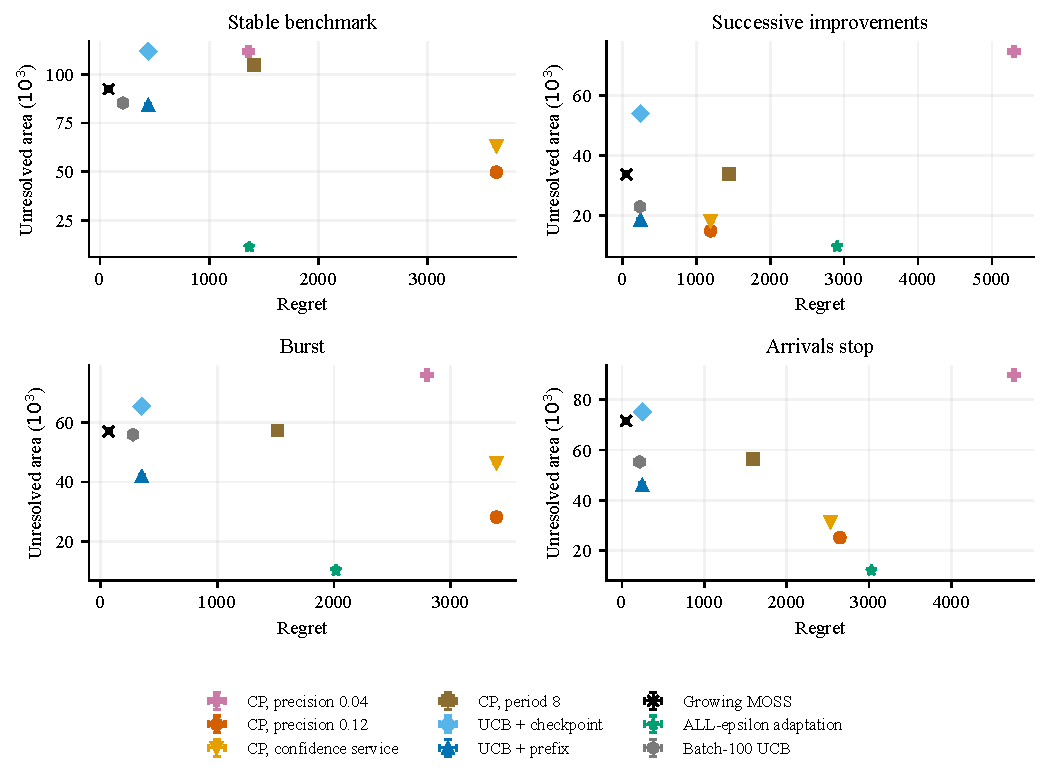
\includegraphics[width=.97\textwidth]{figures/fig_cost_area.pdf}
\caption{Regret and cumulative $\eta$-unresolved area for all nine methods.
Lower values on both axes are preferable. Error bars quantify Monte Carlo
uncertainty, not uncertainty in the theoretical reliability statement.
Neither checkpoint precision nor its allocation variants uniformly dominate
the confidence-based adaptation.}
\label{fig:cost-area}
\end{figure}

\subsection{What the comparisons show}

The finer checkpoint rule leaves between five and eight
$\eta$-unresolved arms on average at the final pull, depending on the
environment. Its unresolved area ranges from 74,820 to 111,784.
This is an observable limitation of the conservative construction, rather
than evidence that arrivals are intrinsically unmanageable at this budget.
The confidence-based adaptation resolves all $\eta$-separated arms by the
end in every replication of these four environments.

The coarser checkpoints reduce area substantially relative to UCB alone,
but can incur much larger regret. Under a stable benchmark, CP-FIFO has
mean regret 3629.9 and area 49,718, compared with 1367.8 and 11,306 for
ALL-$\varepsilon$ adaptation. The paired differences, CP-FIFO minus the
adaptation, are $2262.1$ (standard error $11.7$) for regret and $38{,}411.7$
(standard error $241.9$) for area. The adaptation also improves both
quantities in the burst environment. These comparisons do not support a
general numerical advantage of checkpoint FIFO over a strong
history-retaining identification rule.

In the successive-improvement environment, CP-FIFO instead occupies a
different cost point: regret 1194.7 and area 14,743, compared with 2905.8
and 9525 for the confidence-based adaptation. Here the paired regret
difference is $-1711.0$ (standard error $2.4$), while the area difference is
$5217.7$ (standard error $141.1$). This is consistent with the distinction
between spending pulls to resolve current membership questions and allowing
some questions to be superseded by later arrivals. It is not an estimate
of an optimal Pareto frontier.

Growing-MOSS has the smallest mean regret in all four environments,
between 52.0 and 77.3, while leaving substantially larger unresolved areas.
Low regret therefore provides little evidence of timely set maintenance.
Conversely, the explicit service rules pay for observations of inferior
arms. Reducing service from every second to every eighth pull generally
reduces regret and enlarges unresolved area. Replacing FIFO by the
confidence-driven checkpoint allocation does not uniformly improve either
criterion; allocation and the report's precision both matter.

\begin{figure}[t]
\centering
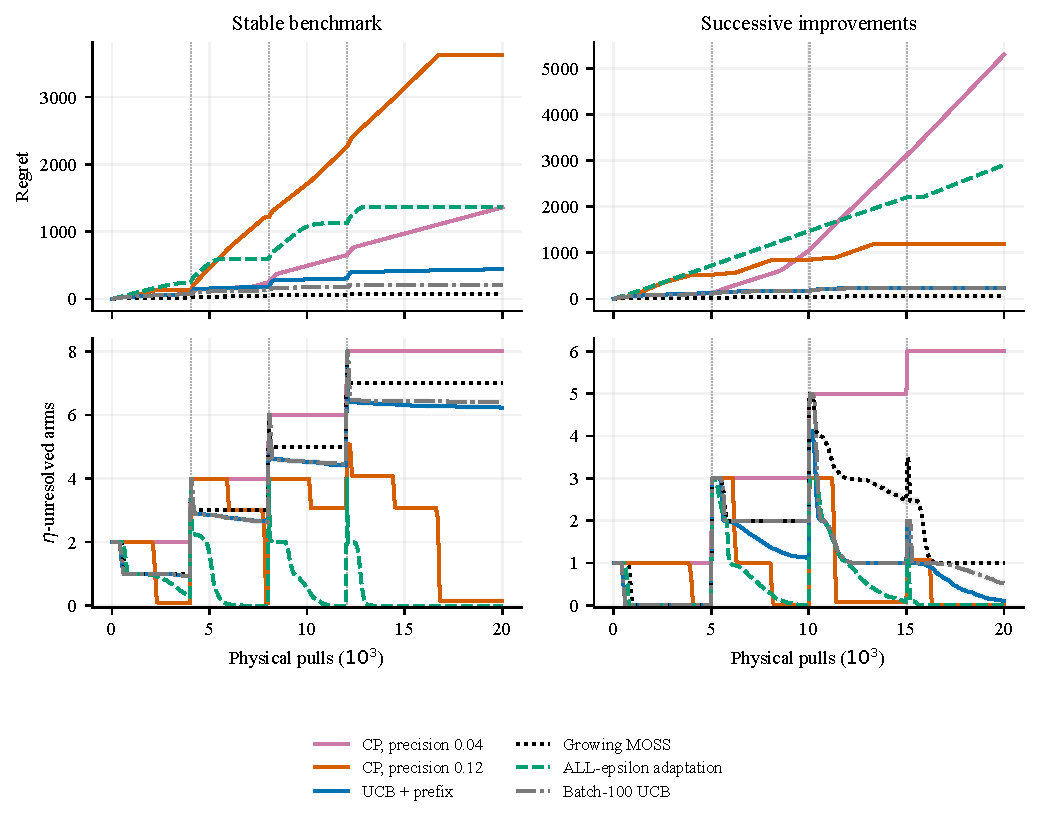
\includegraphics[width=.98\textwidth]{figures/fig_paths_pair1.pdf}
\caption{Mean regret and mean $\eta$-unresolved arm counts at the physical
sampling clock. Bands are 1.96 Monte Carlo standard errors; vertical dotted
lines mark arrivals. Stable and improving benchmarks are shown here;
the other environments appear in the supplement. The main six methods are
displayed; all nine methods and all sampled paths are retained in the released results.}
\label{fig:paths}
\end{figure}

For Batch100-UCB we additionally record the exact decomposition into
within-active regret, admission delay, and loss from previous reward
retirement. Its admission-delay contributions are $0$, $33.92$, $16.00$,
and $22.40$ in the four environments. No historical-retirement deficit
occurred in these runs. The largest discrepancy between total regret and
the sum of the three recorded components was below $3.1\times10^{-12}$.
The corresponding admission and retirement terms are identically zero for
the methods that admit every arm immediately and retain every arm for
reward selection. This accounting avoids attributing every loss outside
within-active learning to arrival delay.

There were no incorrect positive or negative reports in any of the 5760
runs. For one fixed environment and method, zero failures in 160
replications gives a one-sided 95\% upper confidence bound of 0.0186 on
its failure probability. This finite set of diagnostics does not establish
the uniform, all-environment reliability guarantee. Nor do these small
eight-arm experiments validate the asymptotic lower bounds, resolve the
critical logarithmic gap, or establish checkpoint optimality. They show
the practical cost of the conservative quotas and the importance of
comparing retained-history methods under both regret and maintenance
criteria.
\FloatBarrier
\section{Discussion}
\label{sec:discussion}

Reliable maintenance of a relative near-optimal set imposes a cost that is
not visible from allocation regret alone. One arrival can affect many reports
through uncertainty about the common reference level. Repeated improvements
can also make fine discrimination of earlier candidates unnecessary. The
cumulative area criterion measures both effects in the same experiment
and states how much unresolved time a reporting requirement permits.

The strength of the timeliness requirement matters. Sublinear area here means
that the average unresolved \emph{count} vanishes. An application concerned
only with the unresolved proportion, the discovery of one good arm, or a
terminal decision would face a different task. The arrival exponent and
quadratic worst-case area depend on this normalization. Arms in the boundary
band remain in the model: their unresolved time is exempt from the loss, while
every issued label remains subject to correctness.

The finite-time results and eventual consistency also answer different
questions. If arrivals stop, the final arm set is finite, and every arm is
strictly separated from the membership boundary, a revisable multiresolution
version eventually reports the exact set almost surely and has sublinear
expected regret. Its construction and proof are supplied in the supplement.
For the fixed-precision checkpoint implementation, frozen intervals can remain
too wide and an early reporting error need not be corrected, so this consistency
conclusion does not apply. The reward layer retains every available arm and
can still correct allocation.

Our bounds leave a substantive instancewise question. Under arbitrary
overlapping arrivals, heterogeneous boundary distances, and intermediate area
budgets, current information constraints need not describe an attainable causal
allocation. A matching theory would have to price common reference evidence,
unfinished tasks, their possible expiration, and observations already obtained
for reward collection without charging the same observation twice. The
restricted multiple-update theorem leaves that scheduling problem open.
The critical logarithmic gap on an individual smooth schedule and automatic
choice of service precision also remain open.

For practice, the numerical evidence favors examining the two costs together
and comparing methods that retain their history. CP-UCB-AA gives transparent
guarantees, but fixed checkpoints can devote many observations to tasks already
unimportant at a moderate horizon. Confidence-driven adaptations can be much
more efficient, motivating sharper continual-service guarantees for those
rules. A smaller reporting set alone does not establish a resource advantage.

\paragraph{Supplementary material and reproducibility.}
The supplement contains complete proofs, the information-allocation lower
relaxation, the quantile extension, the revisable consistency construction,
and further allocation diagnostics. The numerical package contains the policy
definitions, frozen configurations, every replication, paired Monte Carlo
summaries, figure code, and a source-class parity check. All numerical data in
this article are simulated; no patient-level or other original human-subject
data were used.
\bibliographystyle{plainnat}
\bibliography{references}
\end{document}
